% DIPOLOMARBEITS TABELLEN DEUTSCH ########################
\begin{center}
\textbf{\LARGE DIPLOMARBEIT}

\textbf{DOKUMENTATION}
\end{center}

\begin{tabular}{|p{53mm}|p{110mm}|@{}m{0cm}@{}}
\hline
Namen der \newline Verfasser/innen & Florian Mold \newline Michael Vogler & \\ [0.3cm]
\hline
Jahrgang / Klasse \newline Schuljahr & 5BHIT \newline 2015/16 & \\ [0.3cm]
\hline
Thema der Diplomarbeit & Webplattform für Rechnungserfassung & \\ [0.3cm]
\hline
Kooperationspartner & ELK Fertighaus GmbH & \\ [0.3cm]
\hline
\end{tabular}

\vspace{0.5cm}

\begin{tabular}{|p{53mm}|p{110mm}|@{}m{0cm}@{}}
\hline
Aufgabenstellung & Ziel der Diplomarbeit ist, dass sich die Lieferanten mit ihrer Lieferantennummer bei der Plattform registrieren und warten, bis die Buchhaltung sie freigibt. Danach kann der Lieferant beginnen hochzuladen. Zusätzlich zur Rechnung müssen noch sogenannte Metadaten angegeben werden. Diese beschreiben die Rechnung näher (z.B.: Betrag). Nachdem die Rechnung hochgeladen wurde, erscheint diese in der Buchhaltung. Daraufhin kann ein Buchhalter die Rechnung "holen". Dies bedeutet, dass die Rechnung im PDF-Format mitsamt der Metadaten in Form einer XML-Datei per E-Mail an die automatische Rechnungsverwaltung gesendet wird.  & \\ 
\hline
\end{tabular}

\vspace{0.5cm}

\begin{tabular}{|p{53mm}|p{110mm}|@{}m{0cm}@{}}
\hline
Realisierung & Das System wurde mit der serverseitigen Programmiersprache PHP implementiert. Zusätzlich wurde das Entwicklungsframework Laravel verwendet, um den Entwicklungsprozess zu vereinfachen und zu beschleunigen. Damit die Firma ELK Fertighaus GmbH das System besser in ihre bestehende Struktur integrieren kann, wurde auf eine Oracle-Datenbank gesetzt.  & \\ 
\hline
\end{tabular}

\vspace{0.5cm}

\begin{tabular}{|p{53mm}|p{110mm}|@{}m{0cm}@{}}
\hline
Ergebnisse & Alle Funktionen, die der Auftraggeber vom Projektteam verlangt hat, sind zu seiner Zufriedenheit implementiert. Alle MUSS-Ziele sind in der Anwendung vorhanden und funktional. Auch die optionalen Ziele, nämlich, dass ein Lieferant die Buchhaltung benachrichtigen kann, wenn ein Fehler bei einer seiner Rechnungen aufgetreten ist, wurden implementiert.  & \\
\hline
\end{tabular}
\newpage

\begin{tabular}{|p{53mm}|p{110mm}|@{}m{0cm}@{}}
\hline
Typische Grafik, Foto etc. (mit Erläuterung) & In der untenstehenden Grafik ist die Lieferantenansicht zu sehen. Hier kann eine Rechnung im PDF-Format hochgeladen werden und zusätzlich müssen die Metadaten angegeben werden, bevor der Prozess abgeschlossen werden kann.  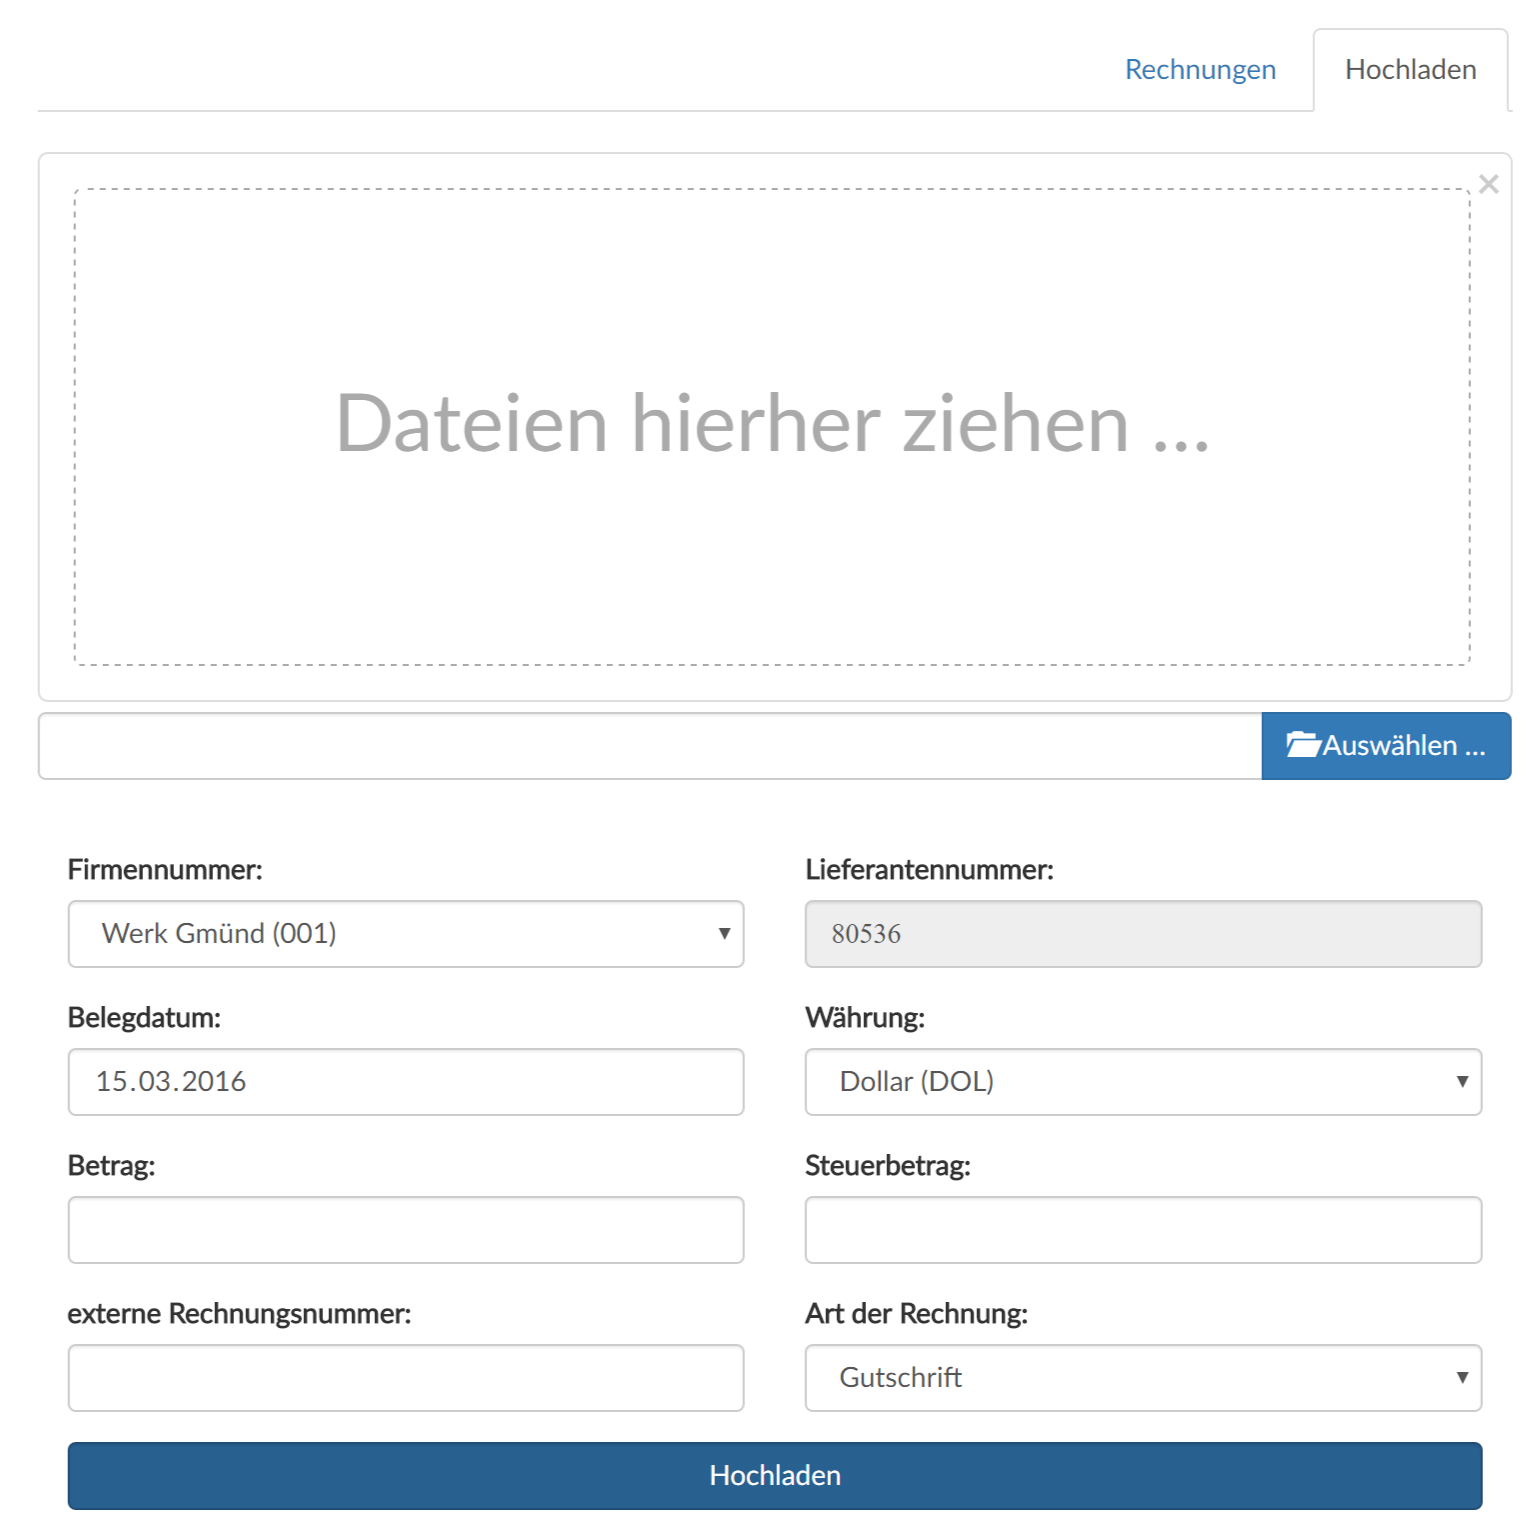
\includegraphics[width=310px, height=320px]{upload.png} & \\
\hline
\end{tabular}

\vspace{0.5cm}

\begin{tabular}{|p{53mm}|p{110mm}|@{}m{0cm}@{}}
\hline
Teilnahme an \newline Wettbewerben, \newline Auszeichnungen & Keine & \\
\hline
\end{tabular}

\vspace{0.5cm}

\begin{tabular}{|p{53mm}|p{110mm}|@{}m{0cm}@{}}
\hline
Möglichkeiten der \newline Einsichtnahme in die \newline Arbeit & Bibliothek der HTL Krems & \\ [0.2cm]
\hline
\end{tabular}

\vspace{0.5cm}

\begin{tabular}{|p{5.3cm}|p{5.28cm}|p{5.29cm}|@{}m{0cm}@{}}
\hline
\vspace{-0.6cm}Approbation \newline (Datum / Unterschrift) & \vspace{-1.1cm} Prüfer/in & \vspace{-1.1cm} Abteilungsvorstand / \newline Direktor/in & \\ [1.9cm]
\hline
\end{tabular}ewline Einsichtnahme in die \newline Arbeit & Bibliothek der HTL Krems & \\ [0.2cm]
\hline
\end{tabular}

\vspace{0.5cm}

\begin{tabular}{|p{5.3cm}|p{5.28cm}|p{5.29cm}|@{}m{0cm}@{}}
\hline
\vspace{-0.6cm}Approbation \newline (Datum / Unterschrift) & \vspace{-1.1cm} Prüfer/in & \vspace{-1.1cm} Abteilungsvorstand / \newline Direktor/in & \\ [1.9cm]
\hline
\end{tabular}